\documentclass{article}

\usepackage[a4paper, total={15cm, 24.5cm}]{geometry}
\usepackage{amsmath}
\usepackage{array}
\usepackage{float}
\usepackage{graphicx}
\usepackage{verbatim}
\title{Data Base 2 Course Notes}
\author{Elia Ravella}
\begin{document}
	\begin{titlepage}
		\maketitle
	\end{titlepage}
	
	\tableofcontents
	\clearpage

	\clearpage
	\part{Transactions}
		\section{Definition and Usages of a Transaction}
			A transaction is usually defined as an \textit{elementary, atomic unit of work  performed by an application}. Transactional systems are those which support transactions. They usually implement a couple of primitives (such as \verb|begin-transaction| and \verb|commit-transaction| or \verb|abort-transaction|) to manage the lifecycle of such an object.

			\paragraph{ACID Properties}
				\begin{enumerate}
					\item Atomicity (all or nothing)
					\item Consistency (only valid states are reachable)
					\item Isolation (transaction should overlap only f they not interfere. The output of cuncurrent transactions should be the same as the output of the very same transactions executed serialized)
					\item Durability (changes are permanent)
				\end{enumerate}
				are the four main properties the are necessary to avoid inconsistent data in a database. Transactional systems tries to embody all these properties in their transaction management mechanism.

			\paragraph{DBMS Modules}
				A Data Base Management System is composed of several interconnected modules:
				\begin{figure}[H]
					\centering
					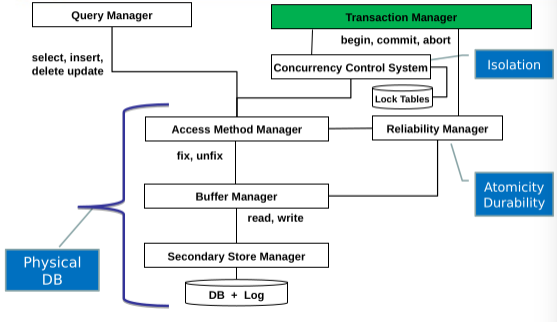
\includegraphics[width = \textwidth]{./images/DBMSModules.png}
					\caption{DBMS modules}
				\end{figure}
				How do those modules interact in order to deliver transactions successfully and which ACID properties they relate to?
				\begin{itemize}
					\item Atomicity and Durability are handled by the \textit{reliability manager}
					\item Isolation is guaranteed by the \textit{cuncurrency control system}
					\item Consistency is managed by the \textit{integrity control system} at query execution time. Obviously in this process the DDL query compiler plays an important role
				\end{itemize}

		\section{Cuncurrency Control}
			DBMSs need cuncurrency. It's pretty straightforward how having multiple transactions executing at the same time increases significantly the throughput of the system. On the other hand, managing cuncurrent systems is a mess. If we add 99\% of cases a DBMS is also distributed across machines, the mess becomes huge. 

			\subsection{Types of Anomalies}
				\begin{itemize}
					\item \textbf{Lost Update}: two transaction write a value in a cell that depends from the previous value (think about an update) but they \textit{both read the same initial value} and so one of the two updates is lost. From the system point of view, the pathologic serie is
						\begin{verbatim}
							r1(x) r2(x) w1(x) w2(x)
						\end{verbatim}
						the first write on \verb|x| is "lost"\footnote{we're assuming that the two updates are dependent.}.
					
					\item \textbf{Dirty Read}: when a transaction rollbacks, it's invalidating all the data it has written or updated. All the reads performed on the values changed\footnote{written} by the aborted transaction are \textit{dirty} in the sense that they'e read an invalid value, so they must be reissued.
						\begin{verbatim}
							r1(x) w1(x) r2(x) abort1 
						\end{verbatim}
					
					\item \textbf{Nonrepeatable Read}: pretty straightforward, this anomaly pops out when two consecutive reads of a value (from a transaction) are allowed to interleave with a write on \textit{that value}. The two read operation will read two different values from the same cell. 
						\begin{verbatim}
							r1(x) r2(x) w2(x) r1(x)
						\end{verbatim}

					\item \textbf{Phantom Update}: Same concept of the Nonrepeatable Read, but this time only a portion of the data read in the first place is modified. The sequence of operation is the same, still.
					\item \textbf{Phantom Insert}: identical as the Nonrepeatable Read, but this time is new data.
				\end{itemize}
				The last three anomalies are conceptually the same thing: someone modifies data thet I've previously read before I've finished using it. This is also similar to the concept or the Lost Update anomaly. In fact, these are all cause by the classic cuncurrent model that's implemented on machines, with the assumptions that writes and reads are so basic operations that they can be easily assumed atomic on their own.

			\subsection{Cuncurrency Theory}
				We define as \textit{Schedule} a serie of basic operations\footnote{reads, writes, aborts, commits} performed by \textit{one or more processes} on \textit{one or more values}. We can define several sets of schedules, discriminating on which properties each one respects. The overall set is
				\begin{figure}[H]
					\centering
					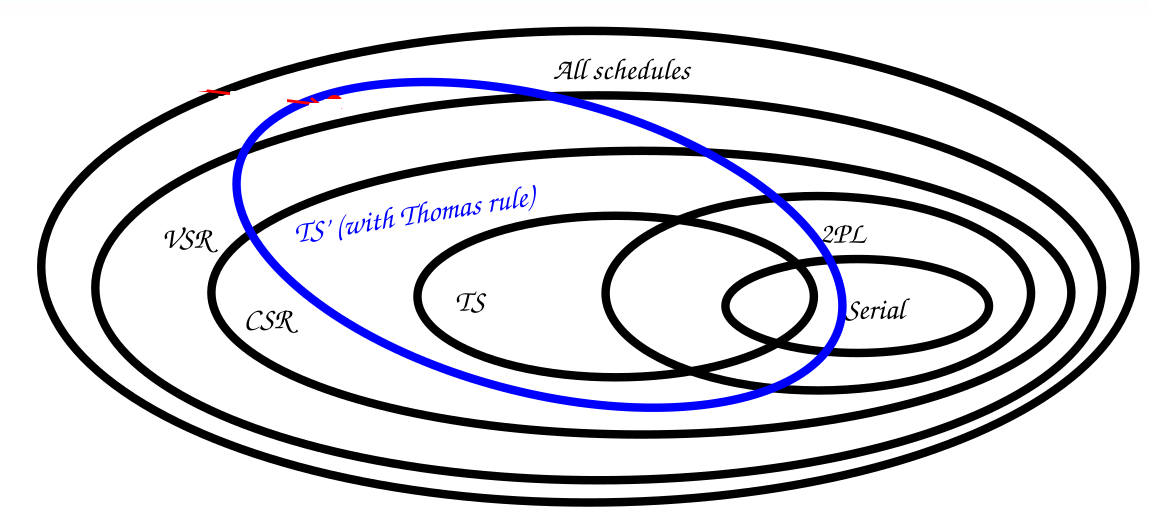
\includegraphics[width = \textwidth]{./images/ScheduleSets.png}
				\end{figure}
				So, there are a lot of sets. Let's analyze all of them
				
				\subsubsection{Serial Schedules}
					Serial schedules are the simplest of all. There's no interleaving of execution threads, all processes start and complete all their operation at once. These kind of schedules do not cause anomalies, but they also \textit{are not cuncurrent}, so they're useless.

					\paragraph{Serializability}
						We love serial schedules from a theoretical point of view. So, a good measure to say if a random schedule is "good" or "bad" for our system can be if we can someway reduce it to a serial equivalent. To do so, we introduce the concept of Serializability, which is a property that holds in concurrent schedules that can be reduced to a serial one without affecting the initial and final states of the DB. We will define less strict serializability equivalence relations for less strict concurrent models.
				
				\subsubsection{View Serializability VSR}
					This set of schedules comprises all the schedules that are view equivalent to a serial one.\\
					Two schedules are view equivalent if
					\begin{enumerate}
						\item They have the same operations
						\item The read operations depends from the same write operations
						\item All variables in the schedules have the same last write operation (same final write property). This can also be rephrased as "the final value of each object is written by the same transaction as if the transactions were executed serially in some\footnote{that can also differ from the order they've been issued.} order"
					\end{enumerate}
					How to check if a schedule is VSR? Simply construct the serial equivalent of the schedule (if S is composed of transactions $T_1, \,T_2, \,T_3$ then the possible serials are  \{$T_1, \,T_2, \,T_3$\} \{$T_1, \,T_3, \,T_2$\} \{$T_2, \,T_3, \,T_1$\} \{$T_2, \,T_1, \,T_3$\} \{$T_3, \,T_2, \,T_1$\} \{$T_3, \,T_1, \,T_2$\}) and verify if there's one among those that produces the same state change.

				\subsubsection{Conflict Serializability CSR}
					Determining if a random query is view serializable is a NP complete problem. We can redefine the equivalence relation we want in order to obtain a reduced set of possible valid schedules that are easier to verify.\\
					A schedule is Conflict Serializable if it's conflict equivalent to a serial schedule.\\
					Two schedules are conflict equivalent if
					\begin{enumerate}
						\item They have the same operations
						\item All conflicts\footnote{conflicts are defined as "couples of operations on the same resource \textit{that contain at least a write operation}"} occur in the same order
					\end{enumerate}
					CSR is a proper subset of VSR. This means that all CSR schedule are also view-serializable, but the viceversa does not hold.\\
					To verify the conflict serializability of a schedule we can resort to a \textit{conflict graph}: it's a graph that has as nodes the transactions, and the edges connect transactions which depends one on another (from the variables point of view)
					\begin{figure}[H]
						\centering
						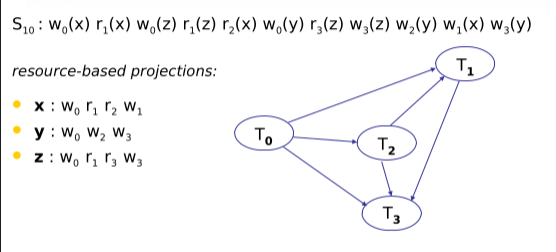
\includegraphics[width = \textwidth]{./images/conflictGraph.png}
					\end{figure}
					The conflict graph is acyclic if and only if the schedule is conflict serializable. If so, it also shows the serial conflic equivalent schedule. 

				\subsubsection{Two Phase Locking 2PL}
					It's not realistic to have all the basic read and write operation before the actual execution of the transaction. CSR and VSR checking methods operates on the \textit{history of operations} but we cannot know them a priori (in most cases). We need methods that can react at the arrival of new operations on line. One of this methods explits a well known technique of concurrency control, locking the resources under request (by a thread / transaction) until the desired operation is finished. The locking mechanism in DBMS uses two locks:
					\begin{enumerate}
						\item Read lock: a transaction requests a read lock when it needs only to read a value from a resource
						\item Write lock: pretty auto esplicative
					\end{enumerate}
					Different lock status are possible, even more locks can be introduced\footnote{Like update lock, that is a read lock "with the intention of writing".}.\\
					2PL is a technique that \textit{imposes a constraint on the usage of locks} in order to provide view (and conflict) serializability. It basically states that \textbf{a transaction cannot require any more lock after releasing one}. The set of schedules that respect this policy is called 2PL and is a \textit{proper subset of CSR}.\\
					2PL (being a proper subset of CSR, also) protects agains
					\begin{itemize}
						\item Lost update anomalies
						\item Phantom update anomalies
						\item Phantom insert anomalies
					\end{itemize}

					\paragraph{Strict 2PL}
						A proper subset of 2PL that also protects from dirty reads is the "strict" version of 2PL, that restricts the shrinking phase (the moment when a transaction releases the locks) to a single moment. This way, there is no chance that a modified variable by a transaction could be read before the commit or abort of the transaction itself.

					\paragraph{Other Locking Mechanism}
						A classic problem of lock based resource control is the presence of deadlocks. To avoid so, we can introduce the so called "Update lock" to the pool of possible locking options: the new status-request table will look like
						\begin{center}
							\begin{tabular}{ c || c | c | c |}
								\hline
								& \multicolumn{3}{| c |}{ \textbf{Resource status}} \\
								\textbf{Type of request} & Shared & Update & Exclusive \\
								\hline
								\hline
								Shared & Granted & Granted & Denied \\
								\hline
								Update & Granted & Denied & Denied \\
								\hline
								Exclusive & Denied & Denied & Denied \\
								\hline
							\end{tabular}
						\end{center}
						Another possible locking mechanism (that addresses the problem of waiting time when waiting for a resource to be unlocked) is \textbf{Hierarchical Locking}, that classify the resources in a hierarchical way (so in a DBMS these could be table over tuple over cell, for example). To cope with this additional complexity in the resource model we must specialize the existing locks in order to take into account the hierarchy of resources. We must introduce \textit{intention} locks, that are a modification of a lock primitive that communicates the need of locking \textit{a subelement} in a given mode. The status request table becomes:
						\begin{center}
							\begin{tabular}{ c || c | c | c | c | c |}
								\hline
								& \multicolumn{5}{| c |}{ \textbf{Resource status}} \\
								\textbf{Type of request} & ISL & IXL & SL & SIXL & XL \\
								\hline
								\hline
								ISL & G & G & G & G & D \\
								\hline
								IXL & G & G & D & D & D \\
								\hline
								SL & G & D & G & D & D \\
								\hline
								SIXL & G & D & D & D & D \\
								\hline
								XL & D & D & D & D & D \\
								\hline
							\end{tabular}
						\end{center}
						In order to obtain a lock on a certain resource, a transaction must hold an equally or more restrictive lock on its parent. In the case of read lock, the hierarchy is $ (ISL, \,IXL \,\geq\, SL, \,ISL) $ and in the case of write locks it's $ (SIXL, \,IXL \,\geq\, IXL, \,SIXL, \, XL) $
					
				\subsubsection{Timestamping}
					Timestamping is an alternative approach to locking, usually called optimistic cuncurrency control\footnote{while locking is usually referred to as "pessimistic" cuncurrency control}. The idea behind is really simple and straightforward: we can timestamp (numerate) events in a way to impose a total ordering of them in the system, and then checked at commit time if there are not "time travelling" things. \\
					The implementation makes use of two counters, one for the Last Read Time and one for the Last Write Time. The policy is: 
					\begin{itemize}
						\item if we want to read a value that has been written \textit{in the future wrt to us} that read is rejected, otherwise is accepted and the Read Time counter will be updated.
						\item If we want to write a value that \textit{has been already read or written in the future} the transaction is killed, otherway is accepted and the Write Time counter is updated.
					\end{itemize}

					\paragraph{Thomas Rule}
						A modification of the write policy (widely used) that can reduce the kill rate of optimistic cuncurrency control is this:\\
						\textit{on a write operation, we reject it \textbf{only if} the value has been read in the future. Otherwise, we just \textbf{skip} the write operation}, since it is obsolete.

					\paragraph{Multiversioning}
						A simple extension of timestampting uses "verisons" of data to avoid killing transactions; the idea is pretty simple, every write does not delete the previous value, but instead it creates a new copy (with its own Write Time counter). Read operations access only the right value for their needs. \textit{This means that there are no invalid reads}. The only operation that is rejected a priori is a write operation on an object that has already been read in the future.\\
						TimeStamping Multiversioning is a set of schedules that is NOT a proper subset of \textit{any} seet we've seen so far. It also comprises non-VSR schedules (much like TimeStamping with Thomas Rule).
	
		\section{Deadlock Detection - Obermarck Algorithm}
			The Obermarck's algorithm is a distributed algorithm that has the aim of creating a "distributed dependency graph" in order to inform all nodes of possible deadlock situations.

			\subsection{Applicability}
				The O's algorithm can be applied only if a certain set of conditions is met:
				\begin{enumerate}
					\item A somewhat centralized contol unit exists (that assigns unique labels, at least)
					\item Transactions can be decomposed in sub-transactions running on other nodes
					\item Super-transactions depend on sub-transactions $\Rightarrow$ "fathers must wait for sons" to proceed and terminate
					\item Two kind of wait-for relationships must exists: 
						\begin{itemize}
							\item Father - Son (or brothers) wait for each other \textit{inside a single node} because of locks etc
							\item Transactions wait for each other \textit{across nodes} through external network calls
						\end{itemize}
				\end{enumerate}

			\subsection{The Algorithm}
				As already said, the idea is that each node exchanges enough information with his neighbours in order to poject onto them a sorta global view of all the dependencies.\\
				In practice, Node A sends info to Node B only if these conditions met:
				\begin{itemize}
					\item A has a transaction that \textit{is waited} from a transaction on another node
					\item A has a transaction that \textit{is waiting} for a transaction on B
					\item The two linked transactions on A that are also linked to B have "descending indexes" (2 waits from 1)
				\end{itemize}
				When a node receives the information about the other transactions from a neighbour, it updates its internal view of the dependency graph and if a cycle is detected, kills a transaction in the cycle.\\

				\paragraph{Example}
					This situation:
					\begin{figure}[H]
						\centering
						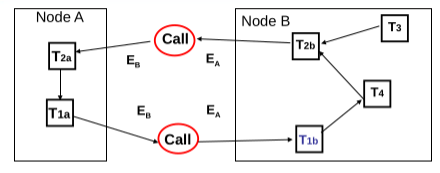
\includegraphics[width = \textwidth]{./images/Obermarck.png}
					\end{figure}
					Node A sees a descending transaction cycle forming: $ E_b \rightarrow T_{2a} \rightarrow T_{1a} \rightarrow E_b = B \,\rightarrow\, 2 \,\rightarrow\, 1 \,\rightarrow\, B $. So it sends it's internal information to B. The same does not happen on B, because the only cycle detected is "in order" ($A \,\rightarrow\, 1 \,\rightarrow\, 2 \,\rightarrow\, A$)\\
					After sending the information to B, A waits. B updates his own dependency graph with all the transactions sent by A, and detectes the $1 \,\rightarrow\, 2 \,\rightarrow\, 1$ circular dependency (that also has $T_4$ in B, but it's not relevant in cycle detection; still, it's one of the potential candidate to be killed in order to break the cycle).



	\part{Memory Management}
		\section{Memory Layers}
			DBMSs run on computers and they have to deal with large datasets. This said, memory management is crucial to deal with DBMS performances. We'll use a reduced model for memory, that only comprises of
			\begin{itemize}
				\item Main memory, structured in \textit{pages}
				\item Secondary mass storage memory, divided in \textit{blocks}
			\end{itemize}
			An I/O operation is defined as "every operation that transfers data from main memory to secondary memory \textit{or viceversa}".
	
			\subsection{Blocks, Tuples}
				How do we map the custom memory structure of a DB schema onto memory? We fix the memory basic block in lenght (this unit is usually referred as as "block" and its read time is usully the basic unit to calculate overall speed of a query) while tuples\footnote{the actual DB records.} are lenght-varying depending on how data is designed at software level.\\
				This difference in lenght calls for the definition of a very simple index, the \textbf{Block Factor} $B = \lfloor \frac{block\, size}{tuple\, size} \rfloor$ that simply is the \textit{number of tuples within a block}.

	
		\section{Access Structures}
			Both in main and in secondary memory we have additional data structures (classic data structures as linked lists, trees, hash tables) that are used to speed up the accessing of memory.\\
			\textbf{Each Table} is stored in \textbf{exactly one primary data structure} and can have \textbf{more than one secondary access structures} but also none.
			\begin{itemize}
				\item The primary structure holds \textit{all the data}. Indipendently from how the data is accessed, there's no pointer to follow if the access is done through a primary structure.
				\item The \textit{secondary} structures are used to \textit{index primary structures} and so they contain mostly pointers to tuples. This means that an extra access to the memory is due, id we're accessing data through a secondary memory structure\footnote{Data can also be stored in secondary structures. We don't care so much though.}. Secondary data access structures are used to speed up the access / search of data in tables, and are \textit{crucial} when it comes to \verb|JOIN| operations, for example.
			\end{itemize}
			We considert three main categories of data structures: sequential, hashed and tree based structures\footnote{corresponding to their relative implementations single linked lists, hash maps and black red trees.}.
	
			\subsection{Data Structures Recap}
				For CS students, data structures should be what we eat at breakfast. I'd like to make a quick recap \textit{considering the fact that we're in the DB realm}, so I'll fly past some aspects while putting the focus on others not in a traditionally way of seeing data structures.\footnote{I've killed english in these two lines.}

				\subsubsection{Sequential Structures}
					We further divide sequential structures in three subcategories:
					\begin{itemize}
						\item Entry sequenced: these are structures organized only by the "arrival order" of tuples
						\item Arrays: index based access structures\footnote{from and exercise point of view, arrays are not that much used}
						\item Sequentially ordered: tuples are ordered (and can be accessed) through a \textit{key}
					\end{itemize}
					Let's analyze these structures with regards to the actual operations that must be performed on them
					\begin{center}
						\begin{tabular}{ c | c | c | c |}
							& Entry sequenced & Array & Sequentially ordered \\
							\hline
							\verb|INSERT| & Efficient & Efficient & Not Efficient \\
							\hline
							\verb|UPDATE| & Efficient & Efficient & Not Efficient for large data sizes \\
							\hline
							Tuple size & Variable & Fized & Variable \\
							\hline
						\end{tabular}
					\end{center}
				
				\subsubsection{Hash Based Structures}
					These structures are \textit{associative structures} that provide access through data by linking it to other piece of data, generally a \textit{well known \textbf{key}} field.\\
					Hash based structures usually make use of "buckets" as as unit of storage (usually the size of a memory block). The buckets of a structure like that are the actual units that are accessed "at once" when an associative access is performed.

					\paragraph{Hashing and Stuff}
						Hash based structures make use of an hash function to identify the bucket (so the tuples) they're accessing at a time. Hash functions are prone to \textit{collisions}, so how are that handled? Two main techniques can be deployed:
						\begin{enumerate}
							\item Open addressing: the tuple is inserted (or searched) in \textit{another bucket} (linearly, recursively with the hash function...). This is NOT the method used in DBMSs.
							\item Separate chaining: a linked list is of bucket is created, with the first bucket as head. If a tuple has the same hash index as the head BUT it's not in the first bucket, then the list is traversed. 
						\end{enumerate}

				\subsubsection{Tree Based Structures}
					The original implementation of SQL indexes made use of trees. In DBMSs, they're pretty powerful tools because they offer a search possibility, through the key of the tree. The most used version of trees (among Binary, Black Red ecc) in databases is the B+ tree: it's a n-ary tree implementation with \textit{many} children per node and \textit{linked leaves}, so to render the all leaves traversal operation linear in the number of leaves.\\
					The distinction Primary/Secondary structure still holds: if a tree is used as a \textit{primary} data structure the leaves will contain directly the data; otherwise, only the \textit{pointer to the data}. Remember: each leaf has a fixed lenght and can contain several blocks\footnote{exercises tips: the "pointers" in a leaf node are just the keys of the tables we're indexing on. So, if the query is selecting that very value, we \textit{don't} have the additional tuple access.}.
	
	\section{Query Optimizer}
		When a query is issued, a module in the DBMS called \textit{query optimizer} takes care of enhancing the query performance, through relational algebraic transformations and reductions. DB1 course concepts as the relational algebra equivalence are largely used here: the less we access the memory\footnote{that's the only performance enhancement we're looking for} the faster the query will complete.
		
		\paragraph{Selectivity}
			Selectivity is a \textit{property} of \textit{filter predicates}, and indicates the probability that any row will satisfy the predicate specified. This value plays a huge role in query optimization: if we have to apply cascading filters, we may want to apply before the more selective, in order to deal with less tuples afterwards. We always assume, if not specified, that the selectivity of a predicate follows an homogeneous distribution. This means that $ S = \frac{1}{N} $ where S is selectivity and N the number of \textbf{values}\footnote{WATCH OUT, it's the number of \textbf{values} not the number of \textbf{tuples}. This means that a binary field will \textbf{\underline{always}} have a selectivity of 0.5, if assumed homogeneously distributed.} available in that field.

		\subsection{Costs of Various Access Patterns}
			\subsubsection{Sequential Scan}
				Well, sequential scan of all blocks. Scan cost = number of blocks (it can eventually be stopped if, for example, we're accessing an ordered field and we have a "less/more than" as a clause).

			\subsubsection{Lookup}
				For lookup is intended a query on a field with an equality or interval predicate associated. We'll analyze the cost of lookups on all structures:

				\paragraph{Primary Hash}
					If the attribute we're costraining in order to perform our selection\footnote{the one in the WHERE clause, to be clear} is the index of the hash table, we can exploit the associative nature of the structure to speed up the search. We have to distinguish if the lookup is done with an equality predicate or an interval predicate
					\begin{itemize} 
						\item Equality lookup: data can be directly accessed from the given constaint, so the overall cost is just $1 + (\text{average overflow chain lenght})$. Usually\footnote{in exercises} there are no overflow chain, so the cost is just unitary.
						\item Interval lookup: usually not supported, but the single values in the interval can be accessed one by one: this makes the overall cost of a interval scan on a primary hash equal to the lenght of the interval itself (with the oppurtune rescaling to the dimension of the blocks).
					\end{itemize}

				\paragraph{Secondary Hash}
					Equality: to the normal $1 + \text{overflow chain lenght}$ we have to add another access to memory (the access to the actual block in the primary storage).\\
					For intervals, same as Primary plus the access to the memory. Again, interval lookups on associative structures are not the best in term of performance.

				\paragraph{Primary B+ Tree}
					All the tree structure must be "traversed downward". This results in an access per level (we are not counting the leaves, for now)
					Reached the leaves, some scenarios are possible: REMEMBER we're assuming that the tree is built on the field we're using to restrict the search
					\begin{itemize}
						\item Equality lookup: if the \textit{single leaf} is needed (equality constraint on unique field) then the access to the leaf is of weight one.
						\item Equality lookup BUT multiple selected tuples: then the accesses to the leaf block\footnote{block are grouped in leaves, that are then mapped to the memory} weights as all the read blocks.
						\item Interval lookup: exactly as the Equality with multiple tuples to return. The first leaf of the interval is reached and then all the blocks are read sequentially. Total cost: $ \{tree\, height\} + \#\{blocks\, accessed\}$.
					\end{itemize}

				\paragraph{Secondary B+ Tree}
					The cost is similar to the primary B+ tree. The leaves this time are to be considered \textit{indipendently from the tree itself}, because they just hold the pointer to the memory block. If we're accessing 13 blocks of memory and a leaf only groups 6 of them at a time, in a 4 levels tree, the total cost of the query is
					\begin{equation}
						\#\{intermediate\, nodes\}\, +\, \#\{total\, leaves\}\, +\, \#\{total\, blocks\}\, =\, 3\, + \lceil\frac{13}{6}\rceil\, + 13
					\end{equation}
					for a total of 20 memory access.\\
					The same reasoning is applicable to the interval queries.

			\subsubsection{Using Statistics}
				Calculating the memory accesses needed to complete a query an important role that's not influenced \textit{by the query itself} but rather \textit{by the data} is the actual number of tuples selected by the interrogation. We've indirectly already used them in the last example for the secondary B+ tree: the fact that we know how many blocks are actually to be retrieved (13) must come from an analysis on the contents of the table.\\
				Selectivity is one of the key indexes when optimizing queries: if an interrogation has multiple predicates, the query optimizer will apply first the \textit{most selective ones} in order to reduce the total number of tuples to be taken. 


			\subsubsection{Join}
				Joins are the most frequent and expensive operations in a database. We can exploit addictional data structure to speed them up.\\
				We'll see three main strategies: nested loops, merge scan and hashed join.

				\paragraph{Nested Loops}
					Classic brutaforce approach to joining. For each tuple of the first table, all the tuples of the second table must be scanned in order to find the ones to join. In the end, the cost is just the product of the number of blocks of each table. WATCH OUT: if it's possible that one of the two tables can be \textit{entirely cached}, then that accesses can be done only one time: the cost reduces to the \textbf{sum} of the blocks of the two tables.\\
					A possible improvement of this simple technique is to combine it with lookups: if we have an additional predicate to the query, we can perform a lookup using the predicate to filter out some of the tuples, and then just join the tuples that satisfy the predicate. I'll add an example from the slide down here, keep in mind most of the data is left out. It's the reasoning the important part.
					\begin{figure}[H]
						\centering
						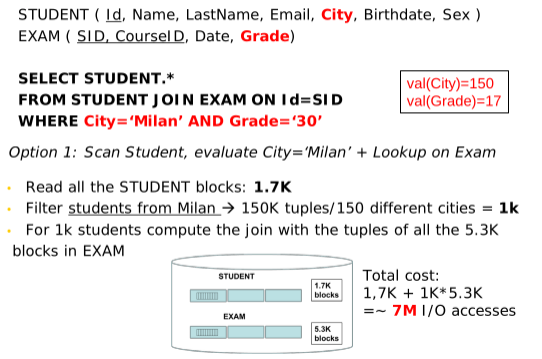
\includegraphics[width = \textwidth]{./images/NestedLoop.png}
					\end{figure}

				\paragraph{Merge Scan}
					This technique can be exploited if the two merging table are ordered on the index we're using to merge. It's intuitive how the sequential nature of the tuples can be used to \textit{progressively merge} all data. In this case, the cost of the join is linear in the number of blocks to be retrieved\footnote{Remember: a B+ is a sequential structure.}. If the merge scan approach gives huge performance improvements, one can also sort the tables and then merge-scan join them. This results in an additional cost (the reorder cost) usually in $N \,\times\, \log(N)$ where N number of blocks to be accessed.

				\paragraph{Hashed Join}
					If two tables are hashed according to the same key of the join operation, then it can be speedupped to cost as a merge scan (so linear in the number of blocks to be read).


	\section{JPA}
		\subsection{Objects and Relations}
			Mapping a relational model typical of a DBMS to an object one, typical of object oriented programming, is no easy task. Moreover, it's \textit{inevitable}: 99\% of web apps rely on a SQL-like database, and they need to use it in a OOP environment. What is the great and very original idea of JPA? Add another software layer that takes care of the ORM\footnote{Object Relational Mapping} and simplifies the passage from one paradigm to another, allowing app programmers to interact with the DB without writing actual DB code.

		\subsection{JPA Main Features and Concepts}
			How do people use JPA\footnote{they don't, by the way} and how is it integrated in a plain Java application? JPA adds these concepts to a standard Java application:
			\begin{itemize}
				\item Entity: a \textit{class} that represents a table in the DB. You will get confused: with "entity", we'll refer both to the class and the instance
				\item Persistence Unit: the \textit{set of classes} (generally a module) that are mapped to the same DB SCHEMA
				\item Persistence Context: all the \textit{actual instanciated objects} of a persistence unit (analogue of the DB INSTANCE)
				\item Managed Entity: an object of an Entity class, in the persistence context. It will reflect all changes from and to the DB
				\item Entity Manager: the interface to the the Persistence Context
				\item Client: a component that can interact with the Persistence Context
			\end{itemize}
			all these "new concepts" are added to the good ol Java language through annotations: if a Java class imports \verb|javax.persistence|\footnote{maybe you'll have to replace Java with Jakarta, I'll let you discover that yourself} it has access to a set of annotations that in the end extends the language to accomodate the mapping to a relational model. The main concepts to keep in mind, among the one presented, are the Entity, the Entity Manager and the concept of Managed Entity.

			\subsubsection{Entity, Managers, Managed Entities}
				When using the "entity" term, we must watch out if it means the entity \textit{class} or the instance in the application. We'll refer to the class as "Entity Class" and to the instance as "Entity" from now on.\\
				An entity is an object\footnote{classic Java object} that gets associated with a \textit{tuple} in the database. If the entity is also \textit{managed} (being the entity manager aware of his presence and linked it to the corresponding tuple) then every changes made to the tuple are reflected to the entity and viceversa. Remember: an entity CAN BE \textbf{UNMANAGED}.  An entity class has features from both the object and the relational worlds: it must have a field marked as primary jey, it must have fields that are annotated to match the table coloums, but it can have methods (as the usual getters, setters, serializers, hashers, iterators-returning ecc ecc). For the correct and complete syntax, use the manual. I'm reporting here just the snippets of\footnote{commented} Java code that is useful to understand how entities are defined and behaves according to relationships.
				\begin{verbatim}
					@Entity
					@Table(name = "EMP")
					public class Employee implements Serializable{
						
					    // the primary key is field-accessed, the identifier is on the field itself
					    @Id
					    @GeneratedValue(strategy = GenerationType.IDENTITY) // this specifies how to handle new items
					    private long EmployeeId
					
					    private int Salary;
					    
					    // this field is property-accessed instead, the annotation is on the getter
					    @Column(name = "SALARY", nullable = false)
					    public int getSalary(){
					        return this.Salary
					    }
					    
					    // many employees in the same department: owning side of a 1:N relationship
					    @ManyToOne
					    @JoinColumn(name = "DEPARTMENT")
					    private Department department;

					    // one employee, some parking lots
					    // careful here: the mappedBy field tells which FIELD maps these entity, it has nothing 
					    //    to do with the DB
					    // the mappedBy should also be present in OneToOne relationships
					    @OneToMany(mappedBy = "employee")
					    private Collection<ParkingLot> parkingLots;

					    // many employees, many projects
					    // M:N relationships want a bridge table (as in ER schemas, they are the composition of two 
					    //    1:N relationships)
					    // this also means that the owner of the relationship is decided by the schema designer
					    @ManyToMany
					    @JoinTable(
					        name = "EMP_PROJ",
					        joinColumns = @JoinColumn(name = "EMP_ID"),
					        inverseJoinColumns = @JoinColumn(name = "PROJ_ID")
					    )
					    private Collection<Project> projects;

					}
				\end{verbatim}

				\paragraph{The Entity Manager}
					The Entity Manager is the interface to ALL the managed objects, and reunites all the functionality to interact with the database. Its interface is super simple:
					\begin{center}
						\begin{tabular}{| m{7.5cm} | m{7.5cm} |}
							\hline
							\verb|public void persist(Object entity)| & makes an entity managed. Remember: \textit{managed} $\neq$ \textit{written in the DB}. \\
							\hline
							\begin{verbatim}public <T> find(
								    Class <T> entityClass, 
								    Object primaryKey
								) 
							\end{verbatim}
								& returns an object from the Persistence Context, searching his primary key. The object will be managed from now on. This triggers also the fetching of the data specified in the fetch policy of the entity class. \\
							\hline
							\verb|public void remove(Object entity)| & removes an entity from the persistence context $\Rightarrow$ from the DB. The plain object in the Java application is still present (pay attention to this) \\
							\hline
							\verb|public void refresh(Object entity)| & re-sync the entity with the DB tuple \\
							\hline 
							\verb|public void flush()| & writes all changes to DB \\
							\hline
						\end{tabular}
					\end{center}
					This interface is easy to use and minimal enough to manage the complex mechanism that is a persistence context. Remember: the \verb|new| keyword \underline{do not add the entity} to the persistence context. 
					\begin{figure}[H]
						\centering
						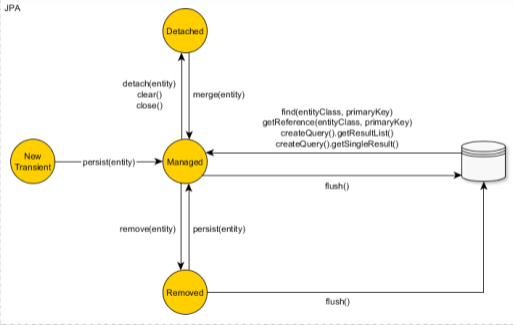
\includegraphics[width = \textwidth]{./images/JPAcalls.png}
						\caption{State transitions and associated calls in the JPA framework.}
					\end{figure}
					Fraternali spends 53 slides jammed of font 10 JPA code to explain how the various type of entity managers behaves wrt the business Java objects (the EJB, Enterprise Java Beans) and wrt the persistence context and the transactions; it's all summed up here:
					\begin{figure}[H]
						\centering
						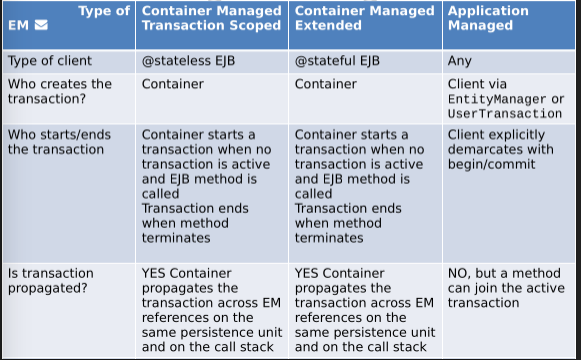
\includegraphics[width = \textwidth]{./images/EMTypes.png}
					\end{figure}
					Again, refer to the manual to find all the right documentation for this stuff.

			\subsubsection{Relationships}
				Mapping relationships between an object oriented worlds and an entity relationship one is kinds strange. Controintuitively, and OO world has \textit{richer} relations between things wrt ER.\\
				An OO relationship is characterized by
				\begin{itemize}
					\item A \textbf{\underline{direction}}: each entity class, in order to access the \textit{other side of the relationship}, may have one or more fields that references the entities on the other side. Practically, the "Author" entity class could reference a "Book" entity class: this is implemented by adding a collection\footnote{usually an implementation of List} of "Books" directly inside the "Author" entity class.
					\item A \textbf{\underline{role}}: at every end of the relation, entities are playing a role. A role represents if you're the source or the target of some data.
					\item A \textbf{\underline{cardinality}}: similar to the cardinality in ER, a relation can be single/multiple on each side. In JPA, a many-to-many relationship model is also available: this will be mapped with an intermediate table on the DB. 
					\item A \textbf{\underline{ownership}}: one of the two entity classes at the end of a relationship is said to be the \textit{owner} of it. The owner is the entity class that \textit{in the db} has the foreign key.
				\end{itemize}

	\section{Active Databases - Triggers}
		Triggers are event based stored procedures in a DBMS. They are SQL statements (usually enriched with some more programming-language-feeling functionalities) associated to an update/insert/delete event on a specific table (or coloumn of a table) and can be used to validate inputs, check and impose invariants, generate and update metadata and so on. They're very powerful.\\
		Triggers follows the ECA paradigm for their definition:
		\begin{itemize}
			\item \textbf{E}vent fires
			\item \textbf{C}ondition is met
			\item then \textbf{A}ction is executed
		\end{itemize}
		watch out for the composite (event + condition) combined.\\
		A full trigger expression is composed of:
		\begin{verbatim}
			create trigger <TriggerName>
			{before | after}
			{insert | delete | update [of <Coloumn>]} on <Table>
			[referencing 
			    {
			        [old table as <OldTAlias>]
			        [new table as <NewTAlias>]
			        [old row as <OldRAlias>]
			        [new row as <NewRAlias>]
			    }
			]
			[for each {row | statement}]
			[when <Condition>]
			<Sql Procedural Statement>
		\end{verbatim}
		where angular brackets indicate literals, square brackets optionality\footnote{all the aliases are optional, alongside the specific coloumn for the updatte table} and curly brackets and vertical bars interchangeability.

		\paragraph{Before and After}
			The "before" and "after" modifier determine when the trigger would be executed with regard to the update being observed.\\
			Before an event means \textit{before the update takes place}, that also mean \textit{before a status change in the schema}. Quick reminder: \underline{before triggers cannot alter the table. They can only adjust the modified rows.} Also, they cannot exactly modify entirely the updating rows: a before trigger can operate in the space of the "new and old" values and tables (see "New and Old" down here).\\
			After triggers are executed after the state of the table has changed.

		\paragraph{Row and Statement}
			Pretty straightforward distinction: a statement \textit{could} affect multiple rows. \verb|for each row| triggers are fired at each update on single rows, while \verb|for each statement| triggers are fired only when the event is catched, even if it affects multiple rows.

		\paragraph{Old and New}
			When dealing with updates, old values and new values must be taken into consideration. SQL generates two variables (old / new for rows, old table / new table for statements) to store the "before and after" values. These variables and accessible values can be very useful when dealine with \verb|when| statements.

		\paragraph{Order of Triggering}
			If several triggers are associated to the same event, they're executed followin this order:
			\begin{enumerate}
				\item BEFORE STATEMENT triggers
				\item BEFORE ROW triggers
				\item state of the table is changed
				\item AFTER ROW triggers
				\item AFTER STATEMENT triggers
			\end{enumerate}

\end{document}



















